\documentclass[25pt, a0paper, portrait, margin=0mm, innermargin=15mm,
     blockverticalspace=15mm, colspace=15mm, subcolspace=8mm]{tikzposter} 

% LATEX PACKAGES
% --------------

\usepackage{graphicx}  % package for inserting images, including .pdf
\usepackage{adjustbox} % package for cropping images
\usepackage[colorlinks=true, urlcolor=blue]{hyperref} % package for url and hyperlinks
\usepackage{wrapfig}

% TITLE, AUTHORS, INSTITUTE
% -------------------------

\title{\textbf{Scaling of biodiversity loss in global coral reef fish}}
\author{Petr Keil*, Nicholas J. Gotelli, Or Givan, Sebastien Villeger,
Valeriano Parravicini, Michel Kulbicki, \\ Jonathan Belmaker \& the GASPAR team}

\institute{*Center for Theoretical Study, Charles University in Prague, Czech Republic \\  
Website: \texttt{\href{www.petrkeil.com}{www.petrkeil.com}},
E-mail: \texttt{\href{mailto:pkeil@seznam.cz}{pkeil@seznam.cz}}}

% THEME SETTING
% -------------

\usetheme{Rays}
%\usecolorstyle[colorPalette=BlueGrayOrange]{Default}
%\useblockstyle{Default}
%\usebackgroundstyle{Default}
\usetitlestyle{Wave}


% HEAD
% ----

\begin{document}
\maketitle
\begin{columns}

% ------------------------
% COLUMN 1 ---------------

\column{0.5}

% AIMS
% ----

\block{Aims}
{
	\begin{enumerate}
		\item To predict loss of coral reef fish diversity 
		based on \textbf{simulated scenarios of loss of coral 
		reef area}. 
		\item To improve methodology of extinction estimation by moving beyond 
		simplistic \textbf{species-area (SAR)} and
		 \textbf{endemics-area (EAR)} relationships that 
		 ignore spatial configuration of habitat loss.
		\item To base the predictions on coral reef 
		\textbf{conservation status, area, remoteness, 
		human pressure and climate}, and also species-specific 
		vulnerabilities.
	\end{enumerate}
	
	\begin{center}
	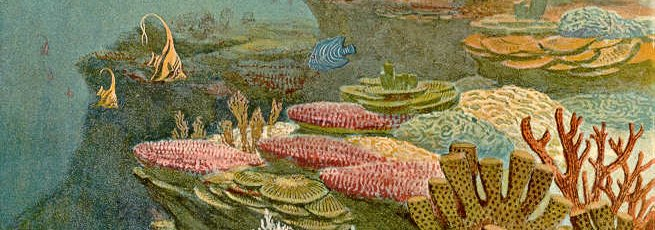
\includegraphics[scale=1.5]{reef.jpg}
	
	\small{"Ancient coral reefs" by Heinrich Harder (1858-1935) - Wikimedia Commons}
	\end{center}
	
	
}

% DATA
% ----

\block{Data}
{
	\begin{itemize}
		\item Species distributional data from the
		 \textbf{GASPAR database} (Kulbicki \textit{et al.} 2013, 
		 Pravicini \textit{et al.} 2013), with 5331 species in 
		 249 grid 5-degree cells that cover 99.76\% of 
		 global coral reef area. 
		\item Data on species-specific \textbf{vulnerability
		to fishing and coral bleaching} 
		(Cheung 	\textit{et al.} 2005, Graham \textit{et al.} 2011).
		\item Data on five cell-specific 
		characteristics (Paravicini \textit{et al.} 2014):
	\end{itemize}
	\begin{center}
		\adjustbox{trim={.0\width} {.0\height} {0.0\width} {.35\height},clip}%
		{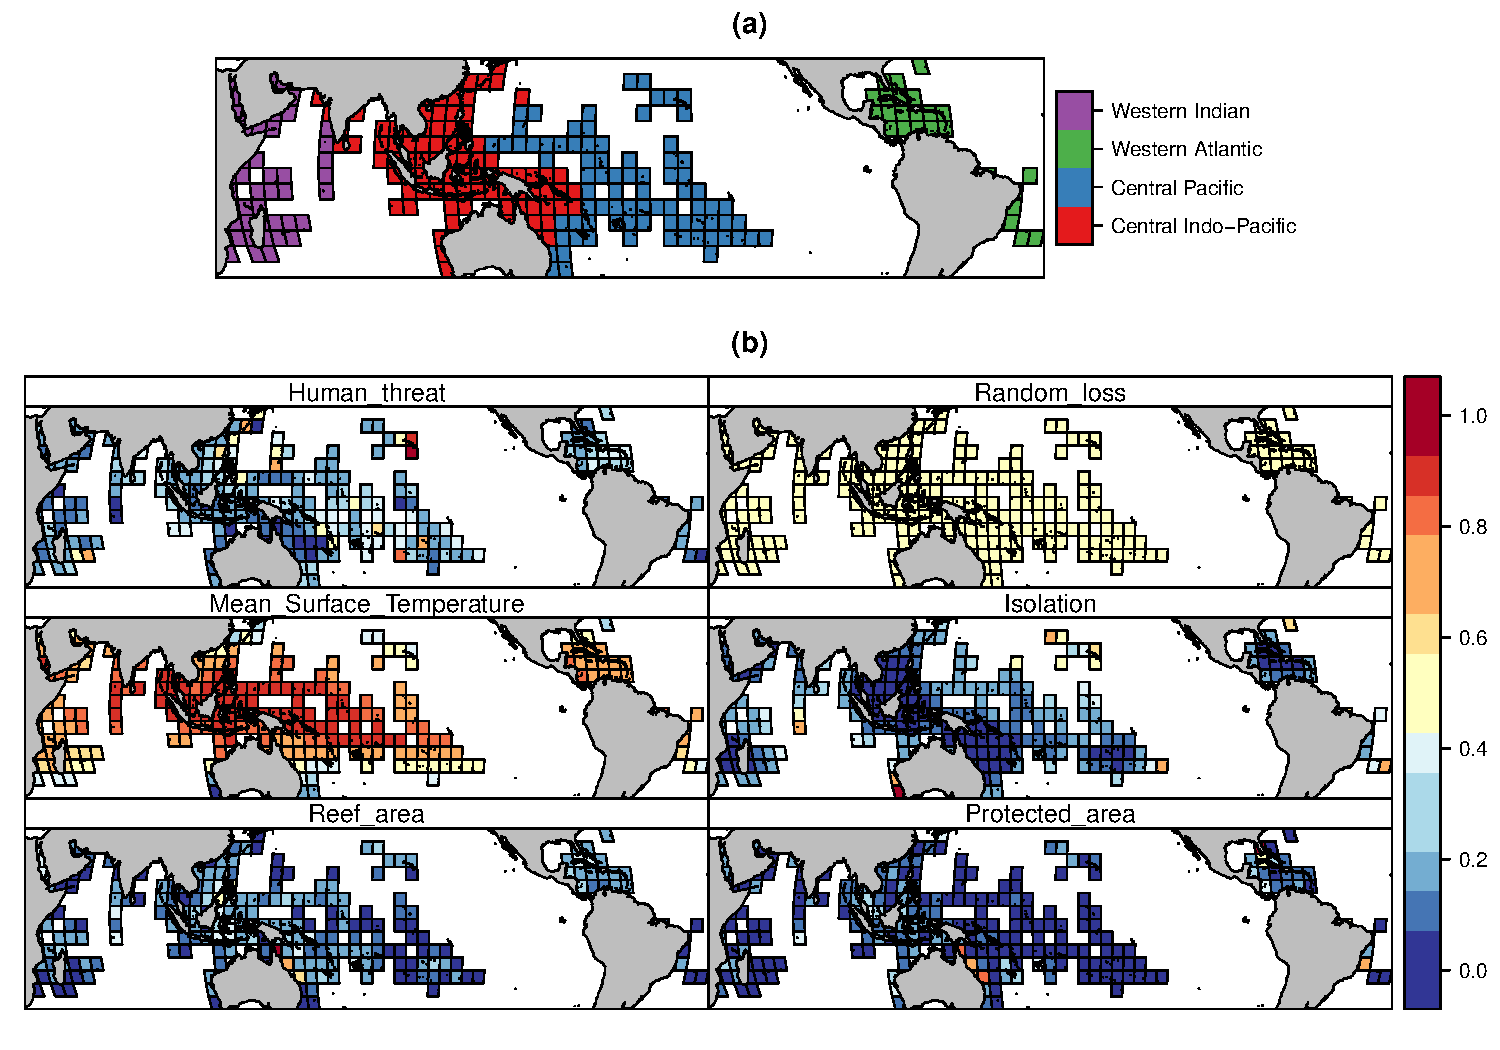
\includegraphics[scale=1.4]{Figure_1.pdf}}	
	\end{center}
}

% METHODS
% -------

\block{Methods}
{
	We run two distinct algorithms to simulate species loss:
	\begin{enumerate}
		\item \textbf{Site removal algorithm}. Large segments 
		of coral reefs are completely destroyed stepwise; in each step 
		all species living in the reef are wiped out.
		\item \textbf{Removing presences in site-species 
		occurrence (SSO) matrix}. We subsequently remove the 
		site-specific species occurrences (SSO), which are the
		presences in the binary site by species
		matrix (panel b). The exact sequence of SSO loss
		depends on the properties both sites and species. 
	\end{enumerate}

	Species loss is summarized by an \textbf{extinction curve} 
	describing relationship between area (or SSO) and number of lost 
	species. Area under the curve (\textbf{AUC}) is our measure 
	extinction magnitude.

	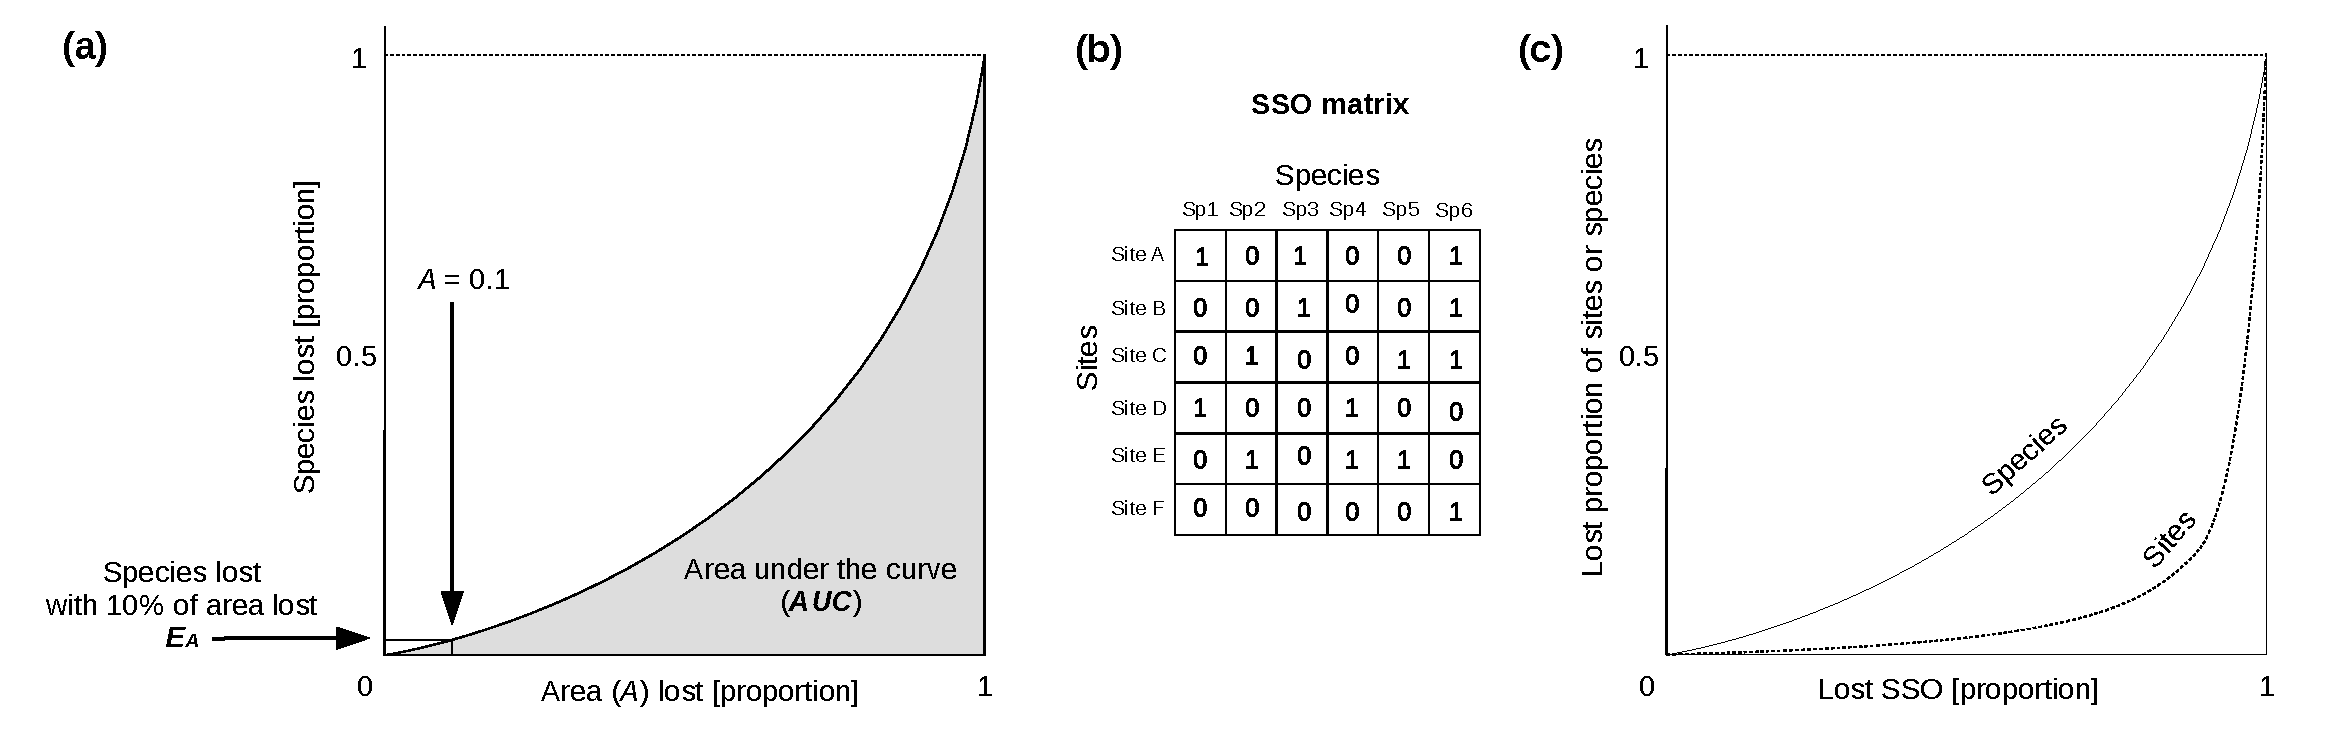
\includegraphics[scale=0.9]{Figure_2.pdf}
}

% ------------------------
% COLUMN 2 ---------------

\column{0.5}

% RESULTS 
% -------

\block{Results 1: Site removal algorithm}
{
  \begin{center}
  \adjustbox{trim={.0\width} {.52\height} {0.0\width} {.0\height},clip}%
		{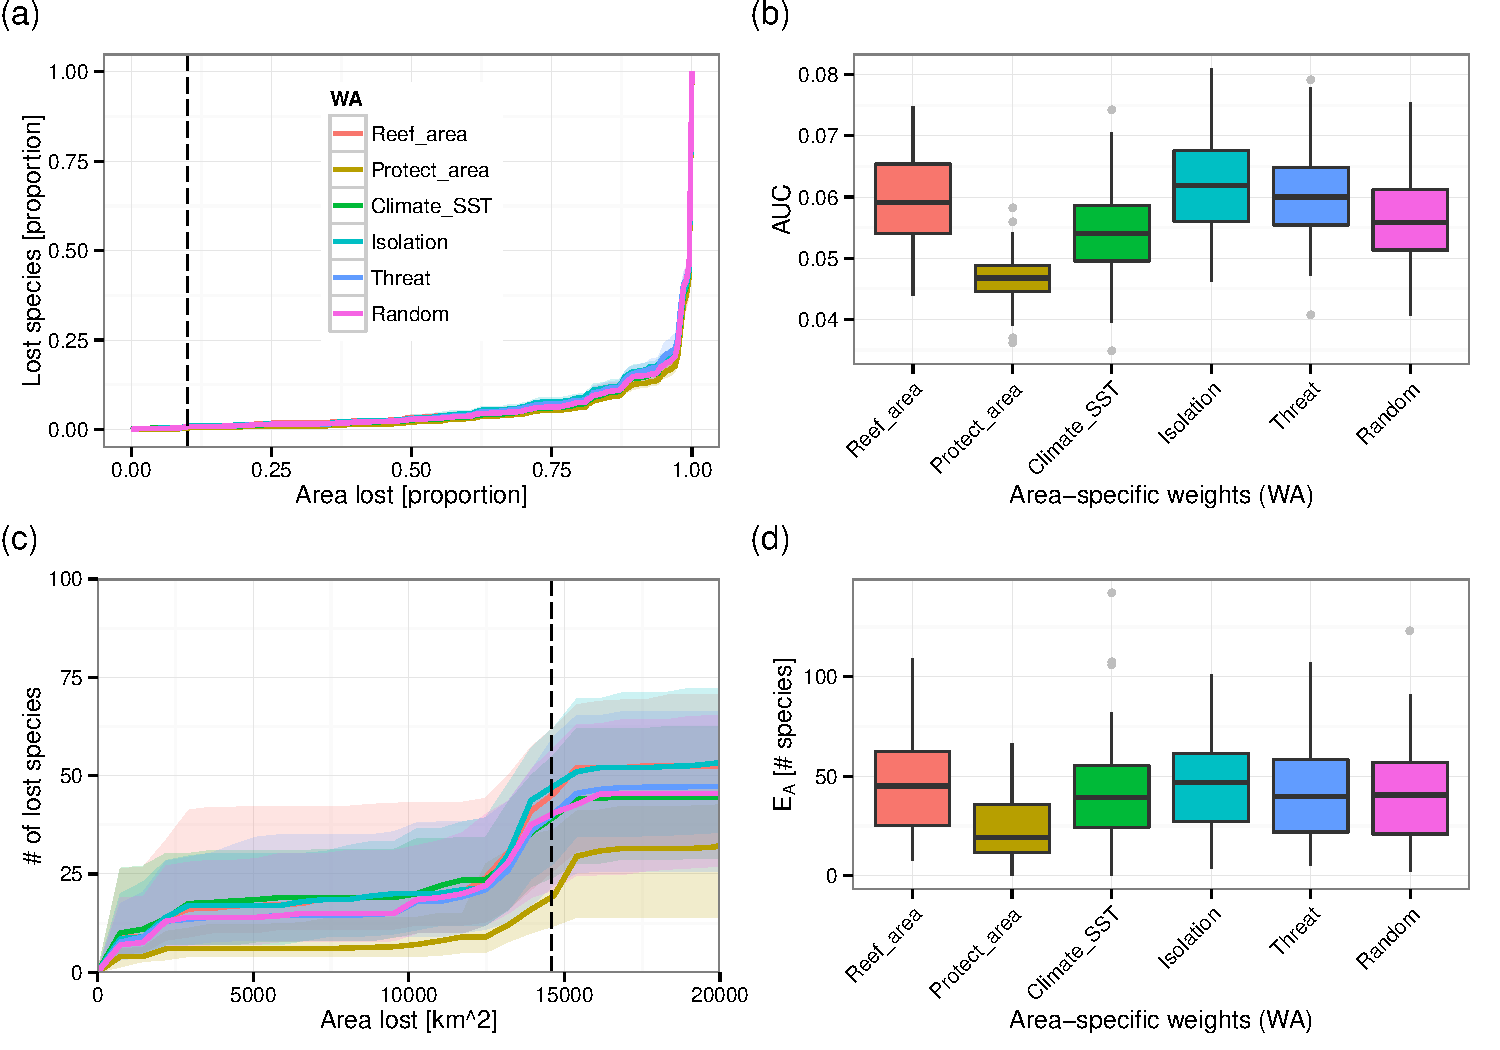
\includegraphics[scale=1.4]{Figure_3.pdf}}
  \end{center}
}

\block{Results 2: Removing presences in site-species occurrence (SSO) matrix}
{
\begin{center}
	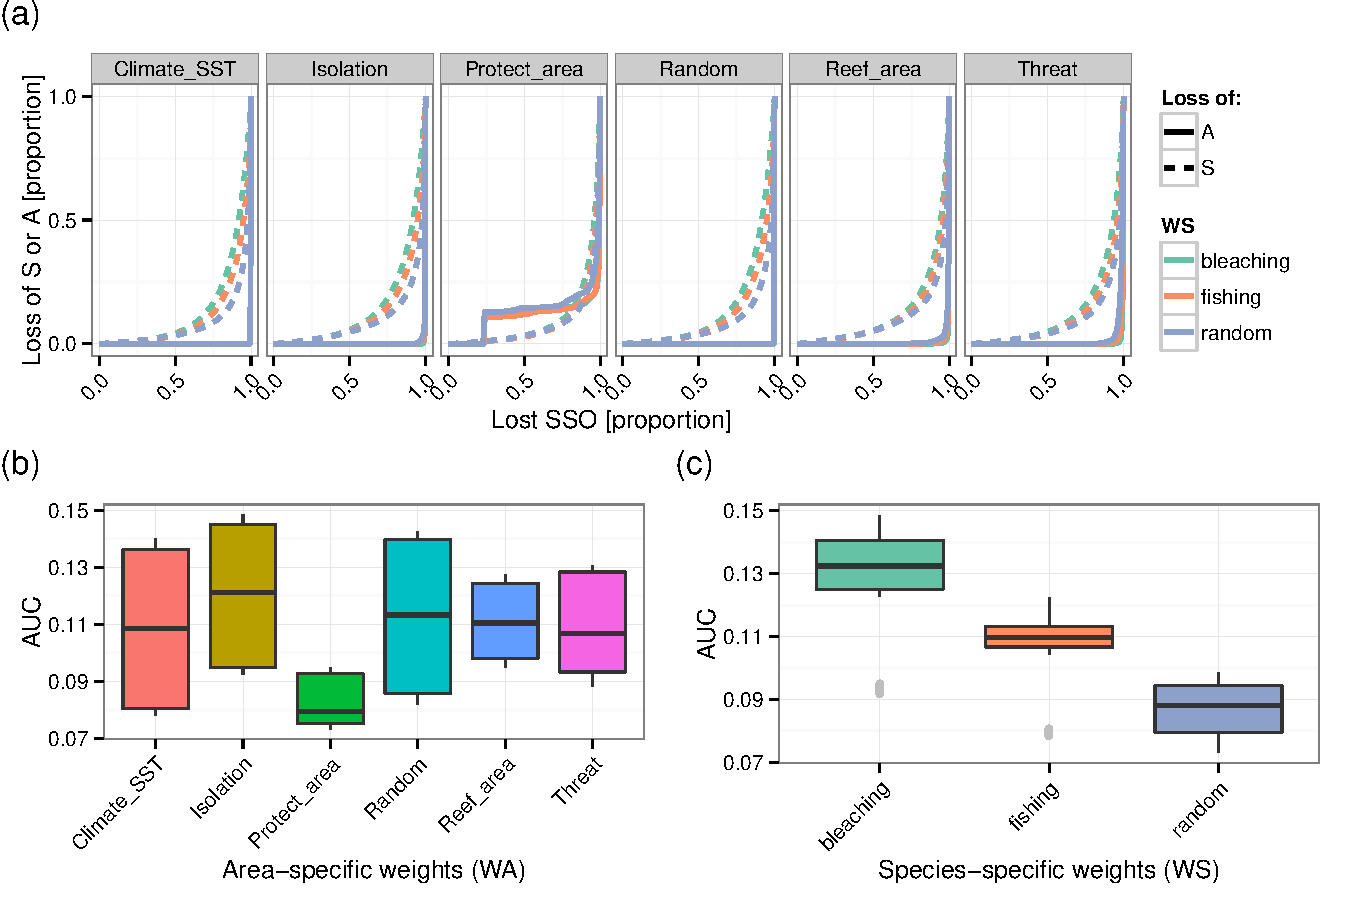
\includegraphics[scale=1.5]{Figure_5.pdf}
\end{center}

}

% CONCLUSIONS
% -----------

\block{Conclusions}
{
\begin{itemize}
  \item Global and regional fish diversity is \textbf{surprisingly difficult to reduce} 
  by removal of compact blocks of coral reefs.
  \item Area loss starting at the most \textbf{isolated} sites leads to most severe 			species loss. 
  \item Area loss that initially avoids \textbf{protected areas} leads to the lowest species loss. This indicates that a non-random 
  and unique part of reef fish diversity is covered by protected areas.
   \item Simulated species loss due to \textbf{fishing and coral bleaching} is 
  higher than random loss. 
  \item Including real-world variables into scenarios of habitat 
  loss give different predictions than simple \textbf{SAR} models. 
\end{itemize}

}

% REFERENCES
% ----------

\block{References}
{
\begin{small}

  \hangindent=2cm Cheung \textit{et al.} (2005) A fuzzy logic expert system to 
  estimate intrinsic extinction vulnerabilities of marine fishes 
  to fishing. \textit{Biological Conservation}, \textbf{124}: 97-111.

  \hangindent=2cm Graham \textit{et al.} (2011) Extinction vulnerability of coral 
  reef fishes. \textit{Ecology Letters}, \textbf{14}: 341-348.

  \hangindent=2cm Kulbicki \textit{et al.} (2013) Global biogeography of reef 
  fishes: a hierarchical quantitative delineation of regions. 
  \textit{PLoS ONE}, \textbf{8}: e81847.

  \hangindent=2cm Paravicini \textit{et al.} (2013) Global patterns and predictors of 
  tropical reef fish species richness. \textit{Ecography}, \textbf{36}: 1-9.

  \hangindent=2cm Paravicini \textit{et al.} (2014) Global mismatch between 
  species richness and vulnerability of reef fish assemblages. 
  \textit{Ecology Letters}, \textbf{17}: 1101-1110.

\end{small}
}

% ACKNOWLEDGEMENTS
% ----------------
\note[targetoffsetx=-8cm, targetoffsety=-9cm, width=25cm, innersep=1cm]
{
    \begin{wrapfigure}{r}{3cm}	
    \vspace{-23pt}
	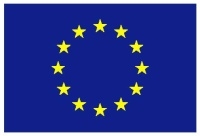
\includegraphics[scale=3]{eu.jpg}
	
	
\includegraphics[scale=3]{fp7.jpg}
	\end{wrapfigure}
	\textbf{Funding:} This research has received funding 
	from the People Programme (Marie Curie Actions) of the EU 7th Framework
	Programme (FP7/2007-2013), REA grant agreement no. 302868.
    
}


\end{columns}

% ----------------
\end{document}
\endinput
%%
%% End of file 
